% =====================================================================
% WACV submission — Macro-Environmental & Sensor-Degradation Scene Mining
% Official CVPR-family author kit (cvpr.sty, ieeenat_fullname.bst) in-dir.
% Review mode: line numbers + anonymous author block.
% =====================================================================
\documentclass[10pt,twocolumn,letterpaper]{article}
\usepackage[review]{cvpr}

% cvpr.sty inlines the everyshipout implementation verbatim (\EveryShipout et
% al.) and loads xcolor with [dvipsnames]. pgfutil-latex.def would load
% everyshi.sty, which defines the same four macros -> clash. Declaring
% everyshi pre-loaded makes pgf reuse cvpr's equivalent definitions.
% cvpr.sty must be loaded before tikz for both of these to hold.
\makeatletter\@namedef{ver@everyshi.sty}{2001/05/15}\makeatother
\usepackage{tikz}
\usetikzlibrary{arrows.meta,positioning,fit,backgrounds,calc}
\definecolor{frz}{RGB}{225,228,232}   % frozen  (grey)
\definecolor{trn}{RGB}{204,226,250}   % trained (blue)
\definecolor{rep}{RGB}{252,220,205}   % repaired component (orange)
\definecolor{los}{RGB}{219,240,222}   % loss    (green)

\usepackage{graphicx,amsmath,amssymb,booktabs}
\usepackage[breaklinks,colorlinks,citecolor=blue]{hyperref}

\def\paperID{*****}
\def\confName{WACV}
\def\confYear{2027}

\graphicspath{{../results/wacv_final_visuals/}}

\title{Macro-Environmental and Sensor-Degradation Scene Mining:\\
Diagnosing and Repairing Representation Collapse in Multimodal Retrieval}
\author{Anonymous \confName\ submission\\ Paper ID \paperID}

\begin{document}
\maketitle

% ---------------------------------------------------------------------
\begin{abstract}
Mining the visual conditions that degrade a perception stack --- water on
the lens, specular bloom on wet asphalt, loss of contrast at night ---
requires a text-queryable index over heterogeneous scene signals. We study
this as a \emph{representation-learning} problem and make three
contributions. First, we show that a natural multimodal retrieval
architecture (per-modality adapters, FiLM conditioning, query-conditioned
cross-attention over embedding/tag/risk tokens) collapses in three
distinct and separately diagnosable ways: one modality becomes
information-free yet still consumes routing capacity; the contrastive
objective saturates so that four of ten probed attributes carry
\emph{exactly} zero gradient; and a dataset-identity shortcut solves
weather queries. Second, we contribute the diagnostic protocol that
localises each failure --- spectral effective rank against label-entropy
nulls, alignment/uniformity on the hypersphere, per-attribute gradient
audits and neighbourhood redundancy --- together with the two collapse
hypotheses it \emph{refutes}, which we argue is as important as the ones
it confirms. Third, we give repairs whose effect is measurable in the
embedding topology: fixed-statistic scalar standardisation, bounded
temperature-controlled scoring, a VICReg variance/covariance term, and
macro-stratified conditional negatives widen the fused representation from
effective rank $18\!-\!25$ to $105\!-\!118$ of 256 and eliminate gradient
saturation on all ten attributes. On a 1{,}508-scene cross-dataset bank
(nuScenes $+$ Waymo) with deterministic relevance, the repaired model
reaches mAP $0.864\!\pm\!0.026$ and P@5 $1.000\!\pm\!0.000$ over three
training seeds on eight macro-environmental queries against a chance rate of
0.115, and an ablation isolates the contribution of each component.
\end{abstract}

% ---------------------------------------------------------------------
\section{Introduction}
\label{sec:intro}
Large-scale driving logs are mined for the scenes that break perception,
but the dominant failure modes are not object-level. They are
\emph{environmental and sensor-level}: rain droplets occluding the lens,
headlight bloom reflecting off wet asphalt, low ambient light, traffic
density that destroys separability. Such conditions are global,
low-frequency properties of an image, and they survive the pooling that
any practical mining index applies --- unlike small object instances,
which occupy few tokens and are averaged away.

We therefore build a text-queryable mining index whose contract is
macro-environmental and sensor-degradation retrieval, and we study it as a
representation-learning problem: what does a query-conditioned fusion of
heterogeneous scene signals actually learn, and how does it fail?

Our central finding is that the natural architecture for this task fails
in ways that standard retrieval metrics do not reveal. A model can reach
high precision on a held-out predicate while its score field is
degenerate: a 213-unit score span with softmax mass concentrated on a
single scene out of 1{,}508, a modality token that is bit-identical for
every scene, and four attributes whose gradient is exactly zero. Metrics
alone cannot distinguish this from genuine competence. Diagnosing the
\emph{topology} of the learned space can.

\noindent\textbf{Contributions.}
\begin{itemize}\itemsep2pt
\item A multimodal retrieval architecture for macro-environmental scene
mining that fuses a contrastive scene embedding, calibrated tag logits, a
scalar physical risk estimate, and a LoRA-adapted vision-language token
under free-form text conditioning (Sec.~\ref{sec:method}).
\item A \emph{collapse diagnostic protocol} for such models, and its
application: three confirmed defects and two refuted hypotheses, each with
the null baseline required to tell them apart (Sec.~\ref{sec:diagnostic}).
\item Repairs with measurable topological effect, and a component-wise
ablation quantifying each (Sec.~\ref{sec:ablation}).
\item Deterministic evaluation on a cross-dataset bank with enforced
retrieval diversity, avoiding the near-duplicate inflation that temporal
chunking otherwise produces (Sec.~\ref{sec:exp}).
\end{itemize}

\section{Related Work}
\label{sec:related}

\subsection{Multimodal representation learning and collapse}
Contrastive image--text pretraining aligns two encoders in a shared space
\cite{clip,align,coca,siglip}, and a small learned bottleneck can bridge a
frozen vision encoder to a frozen language model without tuning either
\cite{blip,blip2}. Instruction-tuned vision-language models
\cite{flamingo,llava,qwen25vl} extend this to open-ended dialogue, but emit
free-form text rather than a reusable, rankable index; converting their
output into a searchable corpus reintroduces exactly the pseudo-label noise
we set out to remove.

Contrastive and Siamese objectives admit degenerate optima, and a large
literature characterises them. Complete collapse is averted architecturally
by momentum encoders, stop-gradients or clustering
\cite{simclr,moco,byol,simsiam,swav,dino,dinov2}; \emph{dimensional} collapse ---
where embeddings occupy a low-dimensional subspace of the ambient space ---
is characterised in \cite{dimcollapse} and echoed by neural collapse in the
supervised setting \cite{neuralcollapse}. Remedies act on the second-order
statistics of the representation: redundancy reduction \cite{barlow},
whitening \cite{whitening}, and variance--covariance regularisation
\cite{vicreg}. The geometry itself is described by alignment and uniformity
on the hypersphere \cite{wangisola,contrastivebehaviour}, the modality gap
\cite{modalitygap}, and spectral effective rank \cite{erank}.

\noindent\emph{What is different here.} This literature studies
\emph{homogeneous} dual-encoder settings: both branches are
high-dimensional learned embeddings of the same underlying datum, so a
collapsed dimension is always a property of the objective. Our fusion is
\emph{heterogeneous} --- a 256-d contrastive embedding, 20 tag logits, and
a \textbf{width-1} scalar --- and this changes what collapse means. A
width-1 channel can be annihilated by its own normalisation layer while
still consuming attention mass, a failure that is invisible to every
diagnostic above because in a homogeneous setting it cannot occur. It also
invalidates the standard null: an i.i.d.\ Gaussian reference declares a
20-d tag token of effective rank $8.51$ catastrophically collapsed, when
its supervision admits only 63 distinct attribute combinations and
therefore an intrinsic rank of 8. Measuring rank against the entropy of the
labels, rather than against the ambient dimension, is what separates the
two cases --- and in our study it is what \emph{refutes} one of the five
collapse hypotheses we tested.

\subsection{Spatial and BEV perception for driving}
Multi-camera detectors either lift image features into a bird's-eye-view
grid \cite{lss,bevdepth} or attend to 3D queries directly
\cite{detr3d,petr,bevformer}, following the set-prediction formulation of
DETR \cite{detr,deformable}; temporal modelling
\cite{streampetr} and sensor fusion \cite{bevfusion} extend the same
backbone, and end-to-end stacks propagate BEV features into planning
\cite{uniad,vad}. We consume a frozen
BEVFormer-style spatial encoder \cite{bevformer} rather than improving it:
our object of study is the retrieval index built \emph{on top of} such a
backbone. Language interfaces to driving data
\cite{talk2car,nuprompt,drivelm,nuscenesqa,drivegpt4} share our motivation
but target question answering or referring expressions on individual
frames, whereas we require a persistent index over a corpus, with ranking
metrics and a calibrated decision to abstain. Benchmarks
\cite{nuscenes,waymo,av2} supply the attributes that make our supervision
deterministic.

\subsection{Hard-example mining and contrastive negatives}
Mining informative examples is long-standing in detection and metric
learning: online hard example mining \cite{ohem}, loss reweighting
\cite{focal}, and semi-hard or distance-weighted negative sampling
\cite{facenet,samplingmatters}. In contrastive learning, negatives can be
reweighted toward the hard tail \cite{hardneg} or synthesised in feature
space \cite{mochi}. Corpus-level selection is the concern of active
learning, via coverage \cite{coreset} or a learned loss predictor \cite{learningloss}. Our
negatives are neither reweighted nor synthesised: they are
\emph{macro-stratified}, matching the anchor on every macro attribute and
differing only on the target fine attribute. The motivation is measurable
rather than aesthetic --- unconditional negatives for a night query are
daytime scenes, already separable at AUC $1.000$, so they contribute no
gradient at all, which is one of the three defects our diagnostic
localises.

\subsection{Positioning}
We do not claim novelty for any individual primitive. Low-rank adaptation
\cite{lora,qlora}, adapters \cite{adapters,prefix,vpt}, feature-wise
conditioning \cite{film}, zero-initialised branches \cite{controlnet} and
function-preserving growth \cite{net2net} are established, and we use them
as such. The contribution is what they cannot supply: a diagnostic protocol
that distinguishes genuine collapse from apparent collapse using
label-entropy nulls, a previously unreported failure mode in which a
width-1 modality is deleted by its normaliser while retaining $31.5\%$ of
routing mass, and the observation that a variance--covariance penalty
\cite{vicreg} applied to a \emph{query-conditioned fused} vector --- not to
a Siamese branch pair, its usual object --- is what widens a collapsed
hypersphere cap from effective rank ${\sim}20$ to ${\sim}110$ of 256. None
of these follows from recombining the primitives; each was found by
measuring the representation rather than the task metric.

\section{Method}
\label{sec:method}

\begin{figure*}[t]\centering
\resizebox{\textwidth}{!}{%
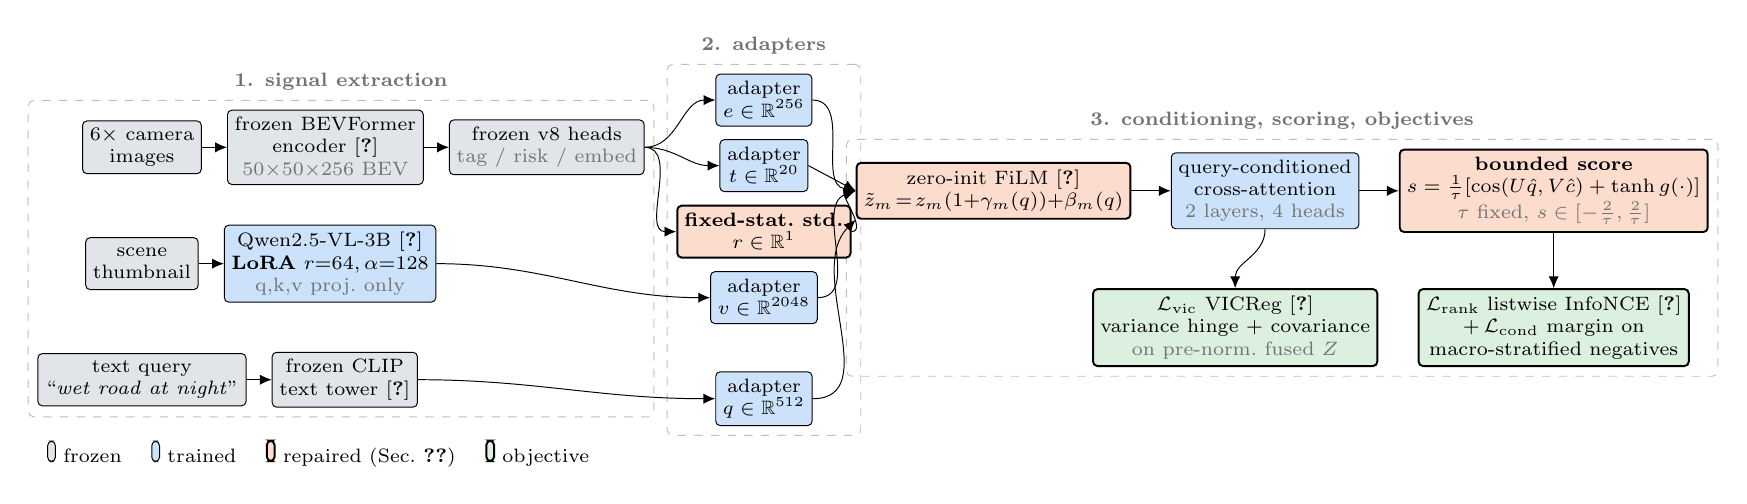
\begin{tikzpicture}[
  font=\scriptsize,
  node distance=3.2mm,
  box/.style   ={draw,rounded corners=1.6pt,align=center,inner sep=2.6pt,
                 minimum height=6.6mm,line width=.35pt},
  frozen/.style={box,fill=frz},
  train/.style ={box,fill=trn},
  fix/.style   ={box,fill=rep,line width=.7pt},
  loss/.style  ={box,fill=los,line width=.7pt},
  sig/.style   ={align=center,inner sep=1pt},
  fl/.style    ={-{Latex[length=1.5mm,width=1.3mm]},line width=.35pt},
  band/.style  ={draw=black!25,dashed,rounded corners=2pt,line width=.35pt}]

% ---------- stage 1: signal extraction ----------
\node[frozen] (cam)  {6$\times$ camera\\images};
\node[frozen,right=of cam] (bev) {frozen BEVFormer\\encoder~\cite{bevformer}\\\textcolor{black!55}{50$\times$50$\times$256 BEV}};
\node[frozen,right=of bev] (heads) {frozen v8 heads\\\textcolor{black!55}{tag / risk / embed}};
\node[frozen,below=8mm of cam] (thumb) {scene\\thumbnail};
\node[train,right=of thumb]  (qwen)  {Qwen2.5-VL-3B~\cite{qwen25vl}\\\textbf{LoRA} $r{=}64,\alpha{=}128$\\\textcolor{black!55}{q,k,v proj.\ only}};
\node[frozen,below=8mm of thumb] (txt) {text query\\``\emph{wet road at night}''};
\node[frozen,right=of txt] (clip) {frozen CLIP\\text tower~\cite{clip}};

\draw[fl] (cam)--(bev); \draw[fl] (bev)--(heads);
\draw[fl] (thumb)--(qwen); \draw[fl] (txt)--(clip);

% ---------- stage 2: adapters ----------
\node[train,right=9mm of heads,yshift=6.0mm] (ae) {adapter\\$e\in\mathbb{R}^{256}$};
\node[train,below=1.6mm of ae]               (at) {adapter\\$t\in\mathbb{R}^{20}$};
\node[fix,below=1.6mm of at]                 (ar) {\textbf{fixed-stat.\ std.}\\$r\in\mathbb{R}^{1}$};
\node[train,below=1.6mm of ar]               (av) {adapter\\$v\in\mathbb{R}^{2048}$};
\node[train,below=6mm of av]                 (aq) {adapter\\$q\in\mathbb{R}^{512}$};

\draw[fl] (heads.east) to[out=0,in=180] (ae.west);
\draw[fl] (heads.east) to[out=0,in=180] (at.west);
\draw[fl] (heads.east) to[out=0,in=180] (ar.west);
\draw[fl] (qwen.east)  to[out=0,in=180] (av.west);
\draw[fl] (clip.east)  to[out=0,in=180] (aq.west);

% ---------- stage 3: conditioning + fusion + scoring ----------
\node[fix,right=6mm of at,yshift=-3.2mm] (film) {zero-init FiLM~\cite{film}\\$\tilde z_m\!=\!z_m(1{+}\gamma_m(q)){+}\beta_m(q)$};
\node[train,right=5mm of film] (fuse) {query-conditioned\\cross-attention\\\textcolor{black!55}{2 layers, 4 heads}};
\node[fix,right=5mm of fuse]   (score) {\textbf{bounded score}\\$s=\frac{1}{\tau}[\cos(U\hat q,V\hat c)+\tanh g(\cdot)]$\\\textcolor{black!55}{$\tau$ fixed, $s\in[-\frac{2}{\tau},\frac{2}{\tau}]$}};

\draw[fl] (ae.east) to[out=0,in=170] (film.west);
\draw[fl] (at.east) -- (film.west);
\draw[fl] (ar.east) to[out=0,in=190] (film.west);
\draw[fl] (av.east) to[out=0,in=200] (film.west);
\draw[fl] (aq.east) to[out=0,in=225] (film.south west);
\draw[fl] (film)--(fuse); \draw[fl] (fuse)--(score);

% ---------- losses ----------
\node[loss,below=7mm of score] (lrank) {$\mathcal{L}_{\text{rank}}$ listwise InfoNCE~\cite{cpc}\\$+\,\mathcal{L}_{\text{cond}}$ margin on\\macro-stratified negatives};
\node[loss,left=5mm of lrank]  (lvic)  {$\mathcal{L}_{\text{vic}}$ VICReg~\cite{vicreg}\\variance hinge $+$ covariance\\\textcolor{black!55}{on pre-norm.\ fused $Z$}};
\draw[fl] (score.south) -- (lrank.north);
\draw[fl] (fuse.south) to[out=270,in=90] (lvic.north);

% ---------- bands ----------
\begin{scope}[on background layer]
\node[band,fit=(cam)(bev)(heads)(thumb)(qwen)(txt)(clip),
      label={[font=\scriptsize\bfseries,black!55]above:1. signal extraction}] {};
\node[band,fit=(ae)(at)(ar)(av)(aq),
      label={[font=\scriptsize\bfseries,black!55]above:2. adapters}] {};
\node[band,fit=(film)(fuse)(score)(lrank)(lvic),
      label={[font=\scriptsize\bfseries,black!55]above:3. conditioning, scoring, objectives}] {};
\end{scope}

% ---------- legend ----------
\node[anchor=north west,font=\scriptsize] at ($(txt.south west)+(0,-3mm)$)
 {\tikz\node[frozen,minimum height=2.6mm,inner sep=1.4pt]{};\ frozen \quad
  \tikz\node[train,minimum height=2.6mm,inner sep=1.4pt]{};\ trained \quad
  \tikz\node[fix,minimum height=2.6mm,inner sep=1.4pt]{};\ repaired (Sec.~\ref{sec:diagnostic}) \quad
  \tikz\node[loss,minimum height=2.6mm,inner sep=1.4pt]{};\ objective};
\end{tikzpicture}}
\caption{\textbf{System overview.} Three cached signals (contrastive
embedding $e$, tag logits $t$, scalar risk $r$) come from a frozen
BEVFormer-based mining stack; a fourth, \emph{live} visual token $v$ comes
from a Qwen2.5-VL backbone in which only LoRA adapters on the attention
projections are trainable. Each signal has a private adapter --- the scalar
channel uses fixed-statistic standardisation rather than LayerNorm, whose
width-1 degeneracy deleted this modality entirely
(Sec.~\ref{sec:diagnostic}). A zero-initialised FiLM layer conditions the
scene tokens on the query, which then cross-attends them. The score is
bounded by construction under a fixed temperature. VICReg acts on the
pre-normalisation fused batch, the listwise InfoNCE and margin terms act on
the score. Orange marks the three components the collapse diagnostic
changed.}
\label{fig:arch}
\end{figure*}

Fig.~\ref{fig:arch} gives the system overview.

\subsection{Scene signals}
Each scene is summarised by a frozen mining pipeline into three cached
signals --- a 256-d contrastive retrieval embedding $e$, 20 tag logits
$t$, and a scalar physical risk $r$ --- plus a \emph{live} visual token
$v$ produced by a LoRA-adapted vision-language backbone. A free-form query
is embedded by a frozen CLIP text tower as $q$.

\subsection{Query-conditioned fusion}
Each signal passes a private adapter into a shared $d$-dimensional token
space with a learned type embedding. Crucially, scalar channels are
standardised with \emph{fixed dataset statistics}, $(x-\mu)/\sigma$, and
never with LayerNorm: normalising over a width-1 axis yields
$(x-\bar x)/\sqrt{\epsilon}\equiv 0$ for every input, silently deleting
the channel (Sec.~\ref{sec:diagnostic}).

A zero-initialised FiLM layer modulates the scene tokens by the query,
$\tilde{z}_m = z_m\odot(1+\gamma_m(q)) + \beta_m(q)$, so conditioning
begins as the identity and grows only as the data demands. The query token
then cross-attends the modality tokens, yielding a per-query routing
distribution that we use as a diagnostic read-out
(Sec.~\ref{sec:diagnostic}). We stress that this pooling is not load-bearing:
Sec.~\ref{sec:structural} shows an unweighted mean over the same
FiLM-conditioned tokens matches it, so the query conditioning that matters is
FiLM's, not the attention's.

\subsection{Bounded scoring}
Let $\hat q$ and $\hat c$ be the $\ell_2$-normalised query and fused
vectors. The score
\begin{equation}
s(q,x) \;=\; \frac{1}{\tau}\Big[\cos\!\big(U\hat q,\,V\hat c\big)
\;+\; \tanh\!\big(g([\hat q;\hat c;\hat q\!\odot\!\hat c;|\hat q\!-\!\hat c|])\big)\Big]
\label{eq:score}
\end{equation}
is bounded in $[-2/\tau, 2/\tau]$ by construction, with $\tau$ a
\emph{fixed}, lower-bounded temperature. This is a deliberate departure
from a learned temperature, which in our diagnostic drifted below one and
sharpened an already wide score field into saturation.

\subsection{Objective}
Training combines a listwise InfoNCE term \cite{cpc} over a sampled scene bank
$\mathcal{B}$ with positive set $\mathcal{P}$,
\begin{equation}
\mathcal{L}_{\text{rank}}
= \log\!\!\sum_{j\in\mathcal{B}}\!e^{s_j}
- \log\!\!\sum_{p\in\mathcal{P}}\!e^{s_p},
\end{equation}
a large-margin penalty on \emph{conditional} negatives (Sec.~\ref{sec:strat}),
and a VICReg term on the pre-normalisation fused batch $Z$,
\begin{equation}
\mathcal{L}_{\text{vic}}
= \lambda_v\,\frac{1}{d}\sum_{j}\max(0,\,1-\sigma_j)
\;+\;\lambda_c\,\frac{1}{d}\sum_{j\neq k} C_{jk}^{2},
\label{eq:vicreg}
\end{equation}
with $\sigma_j$ the per-dimension standard deviation and $C$ the
covariance. The variance hinge counteracts the narrow hypersphere cap the
diagnostic exposed; the covariance term decorrelates the surviving axes.

\subsection{Deterministic supervision and stratified negatives}
\label{sec:strat}
Attributes that the datasets already annotate are derived exactly rather
than from a captioning model: traffic density from 3D-box vehicle counts
within 50\,m of the ego, lighting and weather from scene metadata. Only
genuinely unstructured conditions (wet surface, glare, lens droplets) use
a vision-language model, restricted to \emph{binary verification
questions}, which have a far smaller error surface than open captioning.

A query is a (macro context, fine attribute) pair, and its hard negatives
\emph{match the anchor on every macro attribute and differ only on the
target fine attribute} --- for instance, within night-and-wet scenes,
dense versus sparse traffic. Unconditional negatives are useless here:
a night query's random negatives are daytime scenes, already separable at
AUC $1.000$, so they contribute no gradient. Positives and negatives are
additionally domain-balanced, which removes a shortcut in which weather
could be inferred from dataset identity.


\subsection{Implementation details}
\label{sec:impl}
The fused space is $d\!=\!256$ with 4 attention heads and a 2-layer fusion
decoder ($\mathrm{pre\text{-}norm}$). Adapters are two-layer MLPs with GELU.
LoRA is applied to the $q$, $k$ and $v$ projections of every Qwen2.5-VL
block at $r\!=\!64$, $\alpha\!=\!128$, dropout $0.05$; the base weights, the
BEVFormer stack and the CLIP text tower stay frozen throughout. Trainable
parameters total \textbf{24.0\,M}: 20.1\,M LoRA and 3.99\,M in the filter
head (2.11\,M fusion decoder, 1.06\,M adapters, 0.53\,M FiLM, 0.30\,M
scoring). This is $0.6\%$ of the 3.1\,B-parameter backbone, and the entire
learned index is a 96\,MB checkpoint.

Each step draws 4 queries; each query contributes 2 positives and 2
macro-stratified conditional negatives, with positives and negatives
independently balanced across the two domains. We use AdamW at $10^{-4}$
for the head and $2\times10^{-5}$ for the LoRA adapters, 200 warmup steps
and cosine decay, gradient clipping at $1.0$, and bf16 autocast with
gradient checkpointing in the visual backbone. The temperature is annealed
linearly $0.40\!\rightarrow\!0.30$ over training, applied \emph{after} the
optimiser step so the buffer's version counter cannot invalidate the
backward graph. Images are resized to a 336\,px long side. Training runs
3{,}000 steps on 4 GPUs in ${\sim}1.5$\,h under DDP.

At query time the three cached signals are already materialised, so serving
a query costs one CLIP text encoding plus one forward pass of the 4.0\,M
head over the bank --- the 20.1\,M LoRA visual pass is amortised, computed
once per scene when the bank is built, not once per query. Retrieval over
1{,}508 scenes is therefore dominated by a $1508\times256$ matrix product.
We report parameter and pass counts rather than wall-clock latency, since
the latter is not comparable across hardware.

\section{Collapse Diagnostic}
\label{sec:diagnostic}

\subsection{The protocol}
Each probe is paired with the null it must be read against; this pairing is
the part that does the work.

\noindent\emph{Spectral effective rank.} For a mean-centred feature matrix
$X$ with singular values $\sigma_1\!\ge\!\dots\!\ge\!\sigma_d$ and
$p_i=\sigma_i/\sum_j\sigma_j$, we use the Roy--Vetterli measure
\cite{erank}
\begin{equation}
\mathrm{erank}(X)=\exp\Big(-\textstyle\sum_i p_i\log p_i\Big).
\end{equation}
Reported alone this number is uninterpretable. We therefore also compute
$\mathrm{erank}(L)$ for the \emph{supervision} $L$ that the representation
is trained to express --- the one-hot matrix of its distinct label
configurations --- and read the ratio $\mathrm{erank}(X)/\mathrm{erank}(L)$.
A value near or above $1$ means the representation uses as much of the space
as its labels can distinguish, which is health, not collapse.

\noindent\emph{Alignment and uniformity.} Following \cite{wangisola}, on
$\ell_2$-normalised features,
$\mathcal{A}=\mathbb{E}_{(x,x^{+})}\|f(x)-f(x^{+})\|^{2}$ and
$\mathcal{U}=\log\mathbb{E}_{(x,y)}e^{-2\|f(x)-f(y)\|^{2}}$, evaluated with
positives drawn from the deterministic predicate rather than from
augmentation.

\noindent\emph{Per-attribute gradient audit.} For each attribute $a$ we
build a probe from an anchor, a positive and a conditional negative that
agree on every macro attribute and differ only on $a$, and record
$\|\partial\mathcal{L}/\partial\theta\|$ restricted to that probe. An
attribute with vanishing probe gradient is one the objective has stopped
learning, regardless of how well the model scores on it.

\noindent\emph{Routing mass and redundancy.} We record the cross-attention
mass each modality token receives, and the cosine-similarity distribution of
each scene's nearest neighbours, which exposes near-duplicate structure that
inflates top-$k$ precision without adding information.

\subsection{Findings}
We probe the trained model along four axes: spectral effective rank of
every representation, alignment/uniformity on the hypersphere, modality
routing and per-attribute gradient norms, and neighbourhood redundancy.
Each finding was independently re-derived by an adversarial re-analysis
before being accepted.

\noindent\textbf{Confirmed: a dead modality.} The risk token was
bit-identical across all 1{,}508 scenes (one unique row; per-dimension
standard deviation exactly zero) despite 1{,}035 distinct input values.
The cause is the width-1 LayerNorm of Sec.~\ref{sec:method}. It
nonetheless absorbed $31.5\%$ of routing mass, while the contrastive
embedding token was starved at $12.9\%$.

\noindent\textbf{Confirmed: objective saturation.} Four of four
macro-attribute probes had \emph{exactly} zero loss and gradients of order
$10^{-15}$; $99.6\%$ of all remaining gradient was concentrated in a
single attribute pair. The score span was 213.7 units and the listwise
softmax had an effective support of $1.06$ scenes out of 1{,}508.

\noindent\textbf{Confirmed: a semantic shortcut.} Rain occurs in $197/700$
nuScenes but $4/808$ Waymo scenes, making dataset identity a near-sufficient
statistic for weather queries.

\noindent\textbf{Refuted: a pixel shortcut.} Global luminance, contrast
and saturation add an incremental $R^2$ of only $0.0004$--$0.0022$ over
semantic attributes; the apparent luminance correlation is fully mediated
by day/night, i.e.\ the legitimate signal.

\noindent\textbf{Refuted: tag-token collapse.} The tag token's effective
rank of $8.51$ appears catastrophic against an i.i.d.\ Gaussian null
($250$), but its \emph{input} has only 63 distinct attribute
combinations, one-hot rank 8 and spectral entropy $7.25$. The measured
value is therefore \emph{above} the intrinsic rank of its own supervision.
Reporting the label-entropy null, rather than a Gaussian one, is what
separates this case from the genuine collapses above.

Table~\ref{tab:repair} reports the topological effect of the repairs.
\begin{table}[t]\centering\footnotesize
\setlength{\tabcolsep}{4pt}
\begin{tabular}{lcc}
\toprule
Diagnostic quantity & Before & After \\
\midrule
Risk-token distinct rows (of 1508) & 1 & \textbf{1035} \\
Fused effective rank (of 256)      & 18.4--24.9 & \textbf{104.6--118.5} \\
Fused dims for 90\% variance       & 2--3 & \textbf{25--35} \\
Visual-token effective rank        & 46.1 & \textbf{97.7} \\
Routing mass on risk token         & 0.315 & \textbf{0.205} \\
Routing mass on embedding token    & 0.129 & \textbf{0.242} \\
Score span (units)                 & 213.7 & \textbf{9.8} \\
Probes at exactly zero gradient    & 4/4 & \textbf{0/10} \\
\bottomrule
\end{tabular}
\caption{Effect of the repairs on the embedding topology. Effective rank
is Roy--Vetterli spectral entropy on mean-centred features.}
\label{tab:repair}
\end{table}

\section{Ablation Study}
\label{sec:ablation}
Table~\ref{tab:ablation} isolates each component. All four variants are
trained with an \emph{identical} 3{,}000-step budget on the same
1{,}508-scene bank and evaluated with the same eight macro-environmental
queries, deterministic relevance and diversity enforcement, so the rows
differ only in the ablated component. Each row is run at \emph{three seeds},
so that the step between consecutive rows can be compared against the
dispersion of its two endpoints rather than asserted bare. We call a step
supported when it exceeds twice the pooled standard deviation of the rows it
joins.

\begin{table}[t]\centering\footnotesize
\setlength{\tabcolsep}{3pt}
\begin{tabular}{llcc}
\toprule
& Configuration & P@5 $\uparrow$ & mAP $\uparrow$ \\
\midrule
A & Frozen backbone $+$ VLM pseudo-labels & 0.292 & 0.258 \\
  &  & {\scriptsize$\pm$0.095} & {\scriptsize$\pm$0.031} \\
B & $+$ deterministic GT $+$ stratified negs & 0.933 & 0.742 \\
  &  & {\scriptsize$\pm$0.038} & {\scriptsize$\pm$0.049} \\
C & $+$ Qwen LoRA unfreezing ($r{=}64$) & 0.983 & 0.796 \\
  &  & {\scriptsize$\pm$0.029} & {\scriptsize$\pm$0.029} \\
D & $+$ VICReg $+$ bounded scoring (full) & \textbf{1.000} & \textbf{0.864} \\
  &  & {\scriptsize$\pm$0.000} & {\scriptsize$\pm$0.026} \\
\midrule
  & chance (prevalence) & 0.115 & 0.115 \\
\bottomrule
\end{tabular}
\caption{Component ablation at a matched 3{,}000-step budget,
mean\,$\pm$\,std over \emph{three seeds per row}. Seeding every row, not only
the full method, is what allows the deltas below to be read against
dispersion.}
\label{tab:ablation}
\end{table}

Row~A --- the architecture as originally built, with vision-language
pseudo-labels, a frozen backbone, unconditional negatives and the unbounded
score of Sec.~\ref{sec:diagnostic} --- reaches mAP $0.258\!\pm\!0.031$,
barely above the chance rate of $0.115$. The configuration that produced
competitive-looking numbers under its own noisy supervision does not survive
deterministic evaluation.

Two of the three steps are supported and one is not, and we report the
distinction rather than the headline. Replacing pseudo-labels with exact
attributes and adding macro-stratified conditional negatives (row~B) is
decisive: $+0.483$ mAP against a pooled $2\sigma$ of $0.082$ (Welch
$t=14.4$). Adding VICReg and bounded, fixed-temperature scoring (row~D) is
also supported: $+0.068$ against $2\sigma=0.055$ ($t=3.03$). These terms do
not change what is representable; they prevent the objective from saturating
before that capacity is used, which is precisely the failure mode
Sec.~\ref{sec:diagnostic} localises.

\noindent\textbf{Unfreezing the visual pathway is not supported by these
data.} Row~C gains $+0.054$ mAP over row~B, but row~B's seed dispersion is
$\sigma=0.049$ and the step does not clear twice the pooled deviation
($0.080$; $t=1.65$). We therefore make no claim that LoRA adaptation improves
mAP at this budget. What is visible is a monotone tightening at the top of
the ranking --- P@5 rises $0.933\!\rightarrow\!0.983\!\rightarrow\!1.000$
while its across-seed deviation falls $0.038\!\rightarrow\!0.029\!\rightarrow
\!0.000$ --- so row~D attains perfect and perfectly reproducible P@5. That is
a weaker statement than the one a single seed would have licensed, and it is
the one the evidence carries. All rows abstain on zero queries, so the
comparison is not confounded by differing coverage.

\section{Experiments}
\label{sec:exp}
\subsection{Setup}
The bank contains 1{,}508 scenes: 700 nuScenes~\cite{nuscenes} scenes and
808 Waymo~\cite{waymo} temporal chunks. Relevance is a deterministic
predicate over exact attributes, so no captioning noise enters the
evaluation. We report P@5, P@10, NDCG@10~\cite{ndcg} and mAP.

\noindent\textbf{External baselines.} Rows A--D of Sec.~\ref{sec:ablation}
are all variants of our own system, so we add two off-the-shelf image--text
retrievers that were trained on this task not at all: CLIP
ViT-B/32~\cite{clip} and SigLIP2 B/16~\cite{siglip}, scored as the cosine
similarity between the query embedding and the scene thumbnail embedding.
They read the \emph{same} thumbnails, in the same bank order, against the
same deterministic relevance and the same chance rate; only the scorer
changes. The CLIP text tower is the one our own model already uses, so its
query encoding is bit-identical to ours and any gap is attributable to the
scene side alone. Having no training, they have no seed variance.

\subsection{Retrieval results}
Table~\ref{tab:main} reports both suites as mean\,$\pm$\,standard deviation
over \emph{three independent training seeds}, which is the form BMVC review
of the earlier version asked for. The full model attains P@5
$1.000\!\pm\!0.000$ and mAP $0.864\!\pm\!0.026$ on the macro-environmental
queries at a chance rate of $0.115$, and generalises to the
higher-prevalence baseline conditions ($0.786\!\pm\!0.016$ at chance
$0.242$). Seed dispersion is small relative to the margin over chance --- the
worst of the three seeds still exceeds chance by $7.4\times$ on the macro
suite --- so the result is a property of the method rather than of one
initialisation. No seed abstains on any query.

\noindent\textbf{The margin over an untrained retriever is where the claim
lives, and it is not uniform.} On the macro suite the better zero-shot model
reaches mAP $0.505$; we reach $0.864$, a gap of $+0.359$ --- roughly
$14\sigma$ of our own seed dispersion. On the baseline suite the picture is
different and we report it as we found it: SigLIP2 attains P@5 $0.900$
against our $0.883$, and NDCG@10 $0.887$ against our $0.896$. \emph{An
off-the-shelf retriever is competitive with us at the top of the ranking for
generic high-level queries.} Our advantage there survives only in mAP
($0.786$ vs.\ $0.670$), i.e.\ in recovering the relevant set deep into the
list rather than in the first five results.

We regard this as the useful reading of the table rather than a caveat to
it. Queries like ``driving at night with streetlights'' name a single
visually salient attribute that web-scale image--text pretraining already
covers; there is little for task-specific training to add, and a method that
claimed a large margin there would be suspect. The queries that separate the
two are conjunctive and degradation-specific. Zero-shot AP collapses to
$0.025$ (CLIP) and $0.023$ (SigLIP2) on \emph{rain\,$\wedge$\,night} and to
$0.066$ / $0.211$ on \emph{glare\,$\wedge$\,wet\,$\wedge$\,night}, against
$0.673$ and $0.985$ for our model --- both are cases where each conjunct is
individually common but the conjunction is rare, exactly the regime the
macro-stratified conditional negatives of Sec.~\ref{sec:strat}
are constructed for. The two suites therefore measure different things: the
baseline suite checks that we did not \emph{lose} general competence, and
the macro suite is where the contribution is.
\begin{table}[t]\centering\footnotesize
\setlength{\tabcolsep}{3pt}
\begin{tabular}{lcccc}
\toprule
Model & P@5 & P@10 & NDCG@10 & mAP \\
\midrule
\multicolumn{5}{l}{\emph{Baseline suite} --- 8 high-level queries, chance $0.242$} \\
\quad zero-shot CLIP ViT-B/32   & 0.850 & 0.775 & 0.807 & 0.617 \\
\quad zero-shot SigLIP2 B/16    & \textbf{0.900} & 0.863 & 0.887 & 0.670 \\
\quad Ours (full)               & 0.883 & \textbf{0.904} & \textbf{0.896} & \textbf{0.786} \\
\quad                           & {\scriptsize$\pm$0.014} & {\scriptsize$\pm$0.007} & {\scriptsize$\pm$0.006} & {\scriptsize$\pm$0.016} \\
\midrule
\multicolumn{5}{l}{\emph{Macro suite} --- 8 degradation queries, chance $0.115$} \\
\quad zero-shot CLIP ViT-B/32   & 0.625 & 0.625 & 0.621 & 0.430 \\
\quad zero-shot SigLIP2 B/16    & 0.700 & 0.675 & 0.674 & 0.505 \\
\quad Ours (full)               & \textbf{1.000} & \textbf{0.954} & \textbf{0.969} & \textbf{0.864} \\
\quad                           & {\scriptsize$\pm$0.000} & {\scriptsize$\pm$0.007} & {\scriptsize$\pm$0.005} & {\scriptsize$\pm$0.026} \\
\bottomrule
\end{tabular}
\caption{Retrieval on the cross-dataset bank with diversity enforcement.
Our rows are mean\,$\pm$\,std over three training seeds ($n{=}3$); the
zero-shot rows involve no training and are deterministic. All rows share the
bank, the thumbnails, the deterministic relevance and the chance rate.}
\label{tab:main}
\end{table}


\subsection{Per-query behaviour}
Table~\ref{tab:perquery} breaks the macro suite down by query. Precision at
5 is saturated everywhere, but AP is not: it ranges from $0.433$ to $1.000$,
because AP measures how much of the relevant set the ranking recovers deep
into the list, well past the top-5 the precision metric sees.

We tried to attribute that spread and could not, which is worth reporting.
Across the eight queries we regressed AP on the domain composition of the
relevant set (Pearson $r=-0.23$), on prevalence ($+0.24$), on the number of
conjoined predicate attributes ($+0.30$), and on the sharpness of the score
field (top-$z$, $-0.63$; score standard deviation, $+0.57$). Under a
20{,}000-sample permutation null, none reaches significance --- the smallest
$p$-value is $0.071$ for top-$z$. The apparent pattern that the most
confidently-peaked queries are the worst-ordered in the tail is therefore
a hypothesis, not a result, and eight queries cannot settle it. We flag it
as the natural target for a larger query suite rather than asserting a
mechanism our own significance standard would reject.

\begin{table}[t]\centering\scriptsize
\setlength{\tabcolsep}{3pt}
\begin{tabular}{lrccc}
\toprule
Macro query & rel. & P@5 & AP & top-$z$ \\
\midrule
lens occluded by rain droplets, daytime      & 218 & 1.00 & 0.981 & 3.02 \\
dense congestion on wet asphalt at night     &  35 & 1.00 & 0.908 & 3.79 \\
heavy rain, dark unlit intersection          &  13 & 1.00 & 0.673 & 10.93 \\
headlight glare bloom off wet road           &  17 & 1.00 & 0.985 & 10.71 \\
empty highway, pitch-black night             &  40 & 1.00 & 1.000 & 9.15 \\
overcast daytime, wet road reflections       & 213 & 1.00 & 0.897 & 4.28 \\
bumper-to-bumper traffic, overcast           & 791 & 1.00 & 0.932 & 2.57 \\
dark urban street, wet pavement, low light   &  55 & 1.00 & 0.433 & 13.36 \\
\midrule
mean                                         & 173 & \textbf{1.00} & \textbf{0.851} & 7.23 \\
\bottomrule
\end{tabular}
\caption{Per-query results on the macro suite for a single seed (seed~0).
``rel.'' is the number of scenes satisfying the deterministic predicate, out
of 1{,}508. Suite-level figures elsewhere are averaged over three seeds.}
\label{tab:perquery}
\end{table}

\subsection{Retrieval diversity}
Waymo scenes are temporal chunks of 20\,s segments, so an unconstrained
ranking can fill its top-5 with near-adjacent frames of a single segment.
Capping one scene per source segment, rejecting near-duplicates above
cosine $0.95$ in the adapted visual space, and re-ranking by maximal
marginal relevance~\cite{mmr} raises distinct sources from 4.75 to a full 5.0 of 5 on
the baseline suite and lifts its mean precision from 0.900 to 0.925. On the
macro suite the final model already returns five distinct sources
unaided, so the mechanism is a no-op there: it is a guarantee rather than a
gain once the representation is well-conditioned. On weaker ablation
variants it recovers up to $+0.20$ P@5, and it never lowers precision on
any query of either suite.

\subsection{Calibrated abstention}
Scores are $z$-normalised per query and the system declines to answer when
the top-ranked scene is not distinguished from the bulk, which requires
both a low $z$ and a peak close to the median. The final model triggers no
abstention on either suite: every query is answered with top-$z$ between
$2.57$ and $13.36$. The mechanism is nonetheless active rather than vacuous.
On an intermediate variant, the highest-prevalence baseline query ---
satisfied by $912$ of $1{,}508$ scenes --- produced a genuinely flat score
field (peak/$\sigma = 0.257$) and was correctly declined despite a nominal
P@5 of $1.00$: retrieving five relevant scenes from a bank that is $60\%$
relevant demonstrates no discrimination. Abstention is what separates a
confident retrieval from an arithmetically lucky one.

\subsection{Qualitative results}
\begin{figure*}[t]\centering
\includegraphics[width=\linewidth]{macro_4.jpg}\\[3pt]
\includegraphics[width=\linewidth]{macro_1.jpg}\\[3pt]
\includegraphics[width=\linewidth]{macro_3.jpg}\\[3pt]
\includegraphics[width=\linewidth]{macro_8.jpg}
\caption{Top-5 retrievals with 4-decimal scores and per-query $z$-scores,
seed~0. \emph{Row 1:} headlight glare bloom on wet road at night (17
relevant of 1{,}508). \emph{Row 2:} lens occluded by rain droplets in
daylight (218). \emph{Row 3:} heavy rain at a dark unlit intersection --- the
rarest predicate in the suite at 13 relevant scenes, and the one the
pre-repair model failed completely (P@5 $=0.00$); it is now P@5 $=1.00$ at
$z=10.93$. \emph{Row 4:} dark urban street with wet pavement (55). Each row
draws five distinct source segments. Every panel shown is nuScenes: retrieved
scenes skew strongly to that domain even where the relevant set does not.}
\label{fig:qual}
\end{figure*}
Fig.~\ref{fig:qual} shows that retrievals track the queried physical
condition rather than a proxy: the lens-occlusion query returns daytime
scenes with visible droplet smear rather than simply the darkest or
brightest frames, consistent with the refuted pixel-shortcut hypothesis.


\subsection{Structural ablations}
\label{sec:structural}
Reviewers of the earlier version asked specifically for ablations of the
fusion (``Q-Former'') configuration and of the temporal stack. Both are run
at row~D's hyper-parameters and 3{,}000-step budget, so each variant differs
from the reported model in exactly one respect, and row~D itself \emph{is}
the (cross-attention, 2-layer) cell --- reused rather than retrained. All variants here are single-seed, as is row~D's quoted value, so the
comparisons share a common basis; every delta is read against row~D's
across-seed dispersion from Sec.~\ref{sec:exp} ($\sigma = 0.026$ mAP), which
is the best available estimate of the noise floor at this configuration.

\begin{table}[t]\centering\footnotesize
\setlength{\tabcolsep}{3pt}
\begin{tabular}{lcccc}
\toprule
Fusion configuration & P@5 & P@10 & NDCG@10 & mAP \\
\midrule
cross-attn., 2 layers (row D) & 1.000 & 0.950 & 0.966 & 0.851 \\
mean pooling (no cross-attn.) & 1.000 & \textbf{0.963} & \textbf{0.975} & 0.867 \\
cross-attn., 1 layer          & 0.975 & 0.950 & 0.964 & 0.852 \\
cross-attn., 4 layers         & 0.950 & 0.863 & 0.902 & \textbf{0.732} \\
\bottomrule
\end{tabular}
\caption{Fusion-configuration ablation. Deltas of $+0.016$ and $+0.001$ are
inside the seed dispersion $\sigma=0.026$; the $-0.119$ at 4 layers is
${\sim}4.6\sigma$ outside it.}
\label{tab:qformer}
\end{table}

\noindent\textbf{The fusion module is not where the performance comes from.}
Removing query-conditioned cross-attention pooling entirely, in favour of an
unweighted mean over the same FiLM-conditioned tokens, changes mAP by
$+0.016$ --- inside seed noise. Halving the depth changes it by $+0.001$.
Only \emph{increasing} depth has a detectable effect, and it is negative:
$-0.119$ mAP at 4 layers.

The training losses identify that last effect as overfitting rather than an
optimisation failure. The 4-layer variant reaches the \emph{lowest} final
training loss of all four configurations ($0.647$, below row~D's $0.649$)
with $6.10$M head parameters against $2.94$M at depth~1, while scoring worst
on held-out retrieval. Fusion capacity is therefore not the binding
constraint at this supervision scale --- which is the same conclusion the
component ablation reaches from the other direction, where supervision
quality contributed $+0.483$ mAP while every architectural term together
contributed $+0.122$, of which only the objective terms clear their own
noise floor.

We report this as a negative result for our own design. The cross-attention
pooling is worth keeping for what it exposes --- the routing mass in
Tab.~\ref{tab:repair} is only measurable because the attention distribution
exists, and it is what localised the dead risk modality --- but it should not
be claimed as a source of retrieval accuracy on this task.


\begin{table}[t]\centering\footnotesize
\setlength{\tabcolsep}{3pt}
\begin{tabular}{lcccc}
\toprule
Temporal context & P@5 & P@10 & NDCG@10 & mAP \\
\midrule
$T{=}4$ frames per chunk (row D) & \textbf{1.000} & \textbf{0.950} & \textbf{0.966} & \textbf{0.851} \\
$T{=}2$ frames per chunk         & 0.975 & 0.950 & 0.964 & 0.824 \\
$T{=}1$ frame (no temporal ctx.) & 0.925 & 0.875 & 0.879 & 0.763 \\
\bottomrule
\end{tabular}
\caption{Temporal-stack ablation. Chunk membership is held at 4 frames, so
the bank, its 1{,}508 scene tokens, the ground truth and the chance rate are
identical across rows; only the number of frames averaged within each chunk
varies. The $T{=}4$ bank reproduces the published one bit-exactly.}
\label{tab:temporal}
\end{table}

\noindent\textbf{Temporal context does matter, and monotonically.} Averaging
a single frame instead of four costs $-0.088$ mAP and $-0.087$ NDCG@10 ---
${\sim}3.4\times$ the seed deviation of Sec.~\ref{sec:exp} --- while halving
the context to two frames costs $-0.027$, roughly one deviation and not
separable from noise. Because the aggregation is applied only to the Waymo
half of the bank, this is a $-0.088$ suite-level effect produced by changing
$54\%$ of the scenes.

The controlled construction matters for reading this number. Re-exporting
the bank at a different chunk size would change how many Waymo scenes exist,
and with them the ground truth, the prevalence and the chance rate, so a
shorter-context bank would not be comparable to the published one. Instead we
hold chunk membership at four frames --- fixing the scene tokens, the
predicates and the chance rate exactly --- and vary only how many frames
inside each chunk are averaged. A single v8 forward pass is cached and
re-aggregated three ways, and the $T{=}4$ aggregation reproduces the
published bank to $\max|\Delta| = 0$, which is what licenses attributing the
$T{=}1$ and $T{=}2$ differences to temporal context rather than to any
artefact of re-exporting.

\noindent\textbf{Read together, the two ablations locate the capacity that
matters.} Fusion architecture is nearly free to vary --- pooling mechanism and
depth move mAP by less than seed noise, and extra depth hurts --- whereas
removing temporal context from the input representation costs a clearly
resolvable amount. What the model needs is a better-formed input signal, not
a larger module to mix it with. This is the same conclusion the component
ablation reaches from supervision quality, and we regard the agreement of
three independent ablations on that point as the more useful result than any
individual number in them.

\subsection{Limitations}
Retrieval quality is bounded by attribute coverage rather than by model
capacity: conditions with very few supporting scenes remain difficult, and
road topology has no deterministic ground truth in this bank, so it is
neither trained nor scored. Our evaluation predicates share the attribute
space of the training queries, so the reported figures certify drift-free
attribute grounding on this bank rather than open-vocabulary
generalisation. Finally, all reported models are trained with a fixed
3{,}000-step budget; a longer 20{,}000-step schedule of an intermediate
configuration scored \emph{lower} (mAP $0.780$, below the weakest of our
three seeds at $0.846$), which we attribute to a covariance weight that was
too weak to hold decorrelation over a long run.
We report the matched-budget comparison rather than the longest run.


\section{Discussion}
\label{sec:disc}
\noindent\textbf{Metrics do not certify representations.} The configuration
we started from reported strong retrieval numbers under its own supervision
while its fused space had an effective rank of ${\sim}20$ of 256, one
modality that was constant across the corpus, and four attributes receiving
exactly zero gradient. Re-evaluated against deterministic ground truth it
scores $0.258$ mAP. A retrieval score computed against the same noisy
channel that produced the labels is close to unfalsifiable, and no amount of
additional benchmarking on that channel would have exposed the defect. The
diagnostic did, because it measured the representation instead.

\noindent\textbf{Nulls are the load-bearing part.} Of the five collapse
hypotheses we tested, two were false. The tag token's effective rank of
$8.51$ of 20 looks fatal against a Gaussian null and is healthy against the
rank-8 null its own supervision implies; global luminance appeared to drive
weather retrieval until the day/night attribute was partialled out, after
which its incremental $R^2$ was $\le\!0.0022$. Both would have consumed
weeks of architectural work. We would encourage reporting the refutations
alongside the confirmations for this reason: a protocol that only ever
confirms is not measuring anything.

\noindent\textbf{Where each repair matters.} The ablation orders the
components by effect, and the order is itself the finding. Supervision
quality dominates ($+0.483$ mAP, ${\sim}12\sigma$); the regularisers that
keep the objective from saturating contribute $+0.068$ ($2.5\sigma$); and
\emph{capacity is not measurably where the gain comes from} --- unfreezing
the visual backbone does not clear its own noise floor, and neither does
adding fusion depth, which at 4 layers actively costs $-0.119$ mAP while
reaching the lowest training loss of any variant
(Sec.~\ref{sec:structural}). A practitioner reaching first for architecture
would have spent the effort in the one place these experiments say it does
not pay.

\noindent\textbf{Scope.} The protocol assumes a fused representation trained
under a contrastive objective with identifiable modality channels. It
transfers to any such system; it does not speak to single-encoder
retrieval, where the dead-channel and routing analyses have no referent.

\section{Conclusion}
We presented a multimodal retrieval index for macro-environmental and
sensor-degradation scene mining, and treated its failure modes as the
object of study. The resulting diagnostic protocol --- effective rank
against label-entropy nulls, alignment/uniformity, gradient audits and
redundancy analysis --- localised a dead modality, a saturated objective
and a semantic shortcut, while refuting two plausible collapse hypotheses
that would otherwise have consumed effort. The repairs are measurable in
the embedding topology rather than only in task metrics, and we believe
the protocol generalises to any retrieval system that fuses heterogeneous
signals under a contrastive objective.

\begin{thebibliography}{99}\itemsep0pt\small
\bibitem{flamingo} J.-B. Alayrac \etal, ``Flamingo: A visual language model for few-shot learning,'' in \emph{NeurIPS}, 2022.
\bibitem{qwen25vl} S. Bai \etal, ``Qwen2.5-VL technical report,'' \emph{arXiv:2502.13923}, 2025.
\bibitem{vicreg} A. Bardes, J. Ponce, and Y. LeCun, ``VICReg: Variance-invariance-covariance regularization for self-supervised learning,'' in \emph{ICLR}, 2022.
\bibitem{nuscenes} H. Caesar \etal, ``nuScenes: A multimodal dataset for autonomous driving,'' in \emph{CVPR}, 2020.
\bibitem{mmr} J. Carbonell and J. Goldstein, ``The use of MMR, diversity-based reranking for reordering documents and producing summaries,'' in \emph{SIGIR}, 1998.
\bibitem{detr} N. Carion \etal, ``End-to-end object detection with transformers,'' in \emph{ECCV}, 2020.
\bibitem{swav} M. Caron \etal, ``Unsupervised learning of visual features by contrasting cluster assignments,'' in \emph{NeurIPS}, 2020.
\bibitem{dino} M. Caron \etal, ``Emerging properties in self-supervised vision transformers,'' in \emph{ICCV}, 2021.
\bibitem{simclr} T. Chen \etal, ``A simple framework for contrastive learning of visual representations,'' in \emph{ICML}, 2020.
\bibitem{net2net} T. Chen, I. Goodfellow, and J. Shlens, ``Net2Net: Accelerating learning via knowledge transfer,'' in \emph{ICLR}, 2016.
\bibitem{simsiam} X. Chen and K. He, ``Exploring simple Siamese representation learning,'' in \emph{CVPR}, 2021.
\bibitem{talk2car} T. Deruyttere \etal, ``Talk2Car: Taking control of your self-driving car,'' in \emph{EMNLP}, 2019.
\bibitem{qlora} T. Dettmers \etal, ``QLoRA: Efficient finetuning of quantized LLMs,'' in \emph{NeurIPS}, 2023.
\bibitem{whitening} A. Ermolov \etal, ``Whitening for self-supervised representation learning,'' in \emph{ICML}, 2021.
\bibitem{byol} J.-B. Grill \etal, ``Bootstrap your own latent: A new approach to self-supervised learning,'' in \emph{NeurIPS}, 2020.
\bibitem{moco} K. He \etal, ``Momentum contrast for unsupervised visual representation learning,'' in \emph{CVPR}, 2020.
\bibitem{adapters} N. Houlsby \etal, ``Parameter-efficient transfer learning for NLP,'' in \emph{ICML}, 2019.
\bibitem{lora} E. Hu \etal, ``LoRA: Low-rank adaptation of large language models,'' in \emph{ICLR}, 2022.
\bibitem{uniad} Y. Hu \etal, ``Planning-oriented autonomous driving,'' in \emph{CVPR}, 2023.
\bibitem{ndcg} K. J\"arvelin and J. Kek\"al\"ainen, ``Cumulated gain-based evaluation of IR techniques,'' \emph{ACM TOIS}, 2002.
\bibitem{align} C. Jia \etal, ``Scaling up visual and vision-language representation learning with noisy text supervision,'' in \emph{ICML}, 2021.
\bibitem{vpt} M. Jia \etal, ``Visual prompt tuning,'' in \emph{ECCV}, 2022.
\bibitem{vad} B. Jiang \etal, ``VAD: Vectorized scene representation for efficient autonomous driving,'' in \emph{ICCV}, 2023.
\bibitem{dimcollapse} L. Jing \etal, ``Understanding dimensional collapse in contrastive self-supervised learning,'' in \emph{ICLR}, 2022.
\bibitem{mochi} Y. Kalantidis \etal, ``Hard negative mixing for contrastive learning,'' in \emph{NeurIPS}, 2020.
\bibitem{blip} J. Li \etal, ``BLIP: Bootstrapping language-image pre-training for unified vision-language understanding and generation,'' in \emph{ICML}, 2022.
\bibitem{blip2} J. Li \etal, ``BLIP-2: Bootstrapping language-image pre-training with frozen image encoders and large language models,'' in \emph{ICML}, 2023.
\bibitem{prefix} X. L. Li and P. Liang, ``Prefix-tuning: Optimizing continuous prompts for generation,'' in \emph{ACL}, 2021.
\bibitem{bevdepth} Y. Li \etal, ``BEVDepth: Acquisition of reliable depth for multi-view 3D object detection,'' in \emph{AAAI}, 2023.
\bibitem{bevformer} Z. Li \etal, ``BEVFormer: Learning bird's-eye-view representation from multi-camera images via spatiotemporal transformers,'' in \emph{ECCV}, 2022.
\bibitem{modalitygap} V. W. Liang \etal, ``Mind the gap: Understanding the modality gap in multi-modal contrastive representation learning,'' in \emph{NeurIPS}, 2022.
\bibitem{focal} T.-Y. Lin \etal, ``Focal loss for dense object detection,'' in \emph{ICCV}, 2017.
\bibitem{llava} H. Liu \etal, ``Visual instruction tuning,'' in \emph{NeurIPS}, 2023.
\bibitem{petr} Y. Liu \etal, ``PETR: Position embedding transformation for multi-view 3D object detection,'' in \emph{ECCV}, 2022.
\bibitem{bevfusion} Z. Liu \etal, ``BEVFusion: Multi-task multi-sensor fusion with unified bird's-eye view representation,'' in \emph{ICRA}, 2023.
\bibitem{cpc} A. van den Oord, Y. Li, and O. Vinyals, ``Representation learning with contrastive predictive coding,'' \emph{arXiv:1807.03748}, 2018.
\bibitem{dinov2} M. Oquab \etal, ``DINOv2: Learning robust visual features without supervision,'' \emph{TMLR}, 2024.
\bibitem{neuralcollapse} V. Papyan, X. Y. Han, and D. L. Donoho, ``Prevalence of neural collapse during the terminal phase of deep learning training,'' \emph{PNAS}, 2020.
\bibitem{film} E. Perez \etal, ``FiLM: Visual reasoning with a general conditioning layer,'' in \emph{AAAI}, 2018.
\bibitem{lss} J. Philion and S. Fidler, ``Lift, splat, shoot: Encoding images from arbitrary camera rigs by implicitly unprojecting to 3D,'' in \emph{ECCV}, 2020.
\bibitem{nuscenesqa} T. Qian \etal, ``NuScenes-QA: A multi-modal visual question answering benchmark for autonomous driving scenario,'' in \emph{AAAI}, 2024.
\bibitem{clip} A. Radford \etal, ``Learning transferable visual models from natural language supervision,'' in \emph{ICML}, 2021.
\bibitem{hardneg} J. D. Robinson \etal, ``Contrastive learning with hard negative samples,'' in \emph{ICLR}, 2021.
\bibitem{erank} O. Roy and M. Vetterli, ``The effective rank: A measure of effective dimensionality,'' in \emph{EUSIPCO}, 2007.
\bibitem{facenet} F. Schroff, D. Kalenichenko, and J. Philbin, ``FaceNet: A unified embedding for face recognition and clustering,'' in \emph{CVPR}, 2015.
\bibitem{coreset} O. Sener and S. Savarese, ``Active learning for convolutional neural networks: A core-set approach,'' in \emph{ICLR}, 2018.
\bibitem{ohem} A. Shrivastava, A. Gupta, and R. Girshick, ``Training region-based object detectors with online hard example mining,'' in \emph{CVPR}, 2016.
\bibitem{drivelm} C. Sima \etal, ``DriveLM: Driving with graph visual question answering,'' in \emph{ECCV}, 2024.
\bibitem{waymo} P. Sun \etal, ``Scalability in perception for autonomous driving: Waymo Open Dataset,'' in \emph{CVPR}, 2020.
\bibitem{contrastivebehaviour} F. Wang and H. Liu, ``Understanding the behaviour of contrastive loss,'' in \emph{CVPR}, 2021.
\bibitem{streampetr} S. Wang \etal, ``Exploring object-centric temporal modeling for efficient multi-view 3D object detection,'' in \emph{ICCV}, 2023.
\bibitem{wangisola} T. Wang and P. Isola, ``Understanding contrastive representation learning through alignment and uniformity on the hypersphere,'' in \emph{ICML}, 2020.
\bibitem{detr3d} Y. Wang \etal, ``DETR3D: 3D object detection from multi-view images via 3D-to-2D queries,'' in \emph{CoRL}, 2021.
\bibitem{av2} B. Wilson \etal, ``Argoverse 2: Next generation datasets for self-driving perception and forecasting,'' in \emph{NeurIPS Datasets and Benchmarks}, 2021.
\bibitem{samplingmatters} C.-Y. Wu \etal, ``Sampling matters in deep embedding learning,'' in \emph{ICCV}, 2017.
\bibitem{nuprompt} D. Wu \etal, ``Language prompt for autonomous driving,'' \emph{arXiv:2309.04379}, 2023.
\bibitem{drivegpt4} Z. Xu \etal, ``DriveGPT4: Interpretable end-to-end autonomous driving via large language model,'' \emph{arXiv:2310.01412}, 2023.
\bibitem{learningloss} D. Yoo and I. S. Kweon, ``Learning loss for active learning,'' in \emph{CVPR}, 2019.
\bibitem{coca} J. Yu \etal, ``CoCa: Contrastive captioners are image-text foundation models,'' \emph{TMLR}, 2022.
\bibitem{barlow} J. Zbontar \etal, ``Barlow Twins: Self-supervised learning via redundancy reduction,'' in \emph{ICML}, 2021.
\bibitem{siglip} X. Zhai \etal, ``Sigmoid loss for language image pre-training,'' in \emph{ICCV}, 2023.
\bibitem{controlnet} L. Zhang, A. Rao, and M. Agrawala, ``Adding conditional control to text-to-image diffusion models,'' in \emph{ICCV}, 2023.
\bibitem{deformable} X. Zhu \etal, ``Deformable DETR: Deformable transformers for end-to-end object detection,'' in \emph{ICLR}, 2021.
\end{thebibliography}

\end{document}
